\documentclass{homework}
\usepackage{cancel}
\usepackage{amsthm}
\usepackage{cleveref}
\usepackage{upgreek}
\usepackage[framed]{mcode}
\usepackage{mathrsfs}
\usepackage{units}
\usepackage{pgf,tikz}
\usetikzlibrary{arrows}
\usetikzlibrary{matrix}
\newtheorem{lemma}{Lemma}

\title{Kevin Joyce}
\course{Math 564 - Hermetian Analysis}
\author{Kevin Joyce}
\docdate{\today}
\begin{document} 
\newcommand{\figref}[1]{\figurename~\ref{#1}}
\renewcommand{\bar}{\overline}
\renewcommand{\hat}{\widehat}
\renewcommand{\SS}{\mathcal S}
\newcommand{\eps}{\varepsilon}
\newcommand{\TTheta}{\overline{\underline \Theta} }
\newcommand{\del}{\partial}
\newcommand{\approxsim}{\overset{\cdotp}{\underset{\cdotp}{\sim}}}

\problem{{\bf D'Angelo 1.13} Assume $a\in \RR, b \in \CC$, and $c>0$.  Find the minimum of the Hermitian polynomial R:
$$
  R(t,\bar t) = a + bt + \bar b\bar t +c |t|^2.
$$
}

\begin{solution}
Note 
\begin{align*}
  R(t,\bar t) 
  &= c\left(t + \bar b/c\right)\bar{\left(t + \bar b/c\right)} - |b|^2/c + a \\
  &\stackrel{*}= c|t + \bar b/c|^2 + (a-|b|^2/c) \\
  &\ge (a - |b|^2/c)
\end{align*}
for all $t \in \CC$. Moreover, if $t = -\bar b/c$, then $R(t,\bar t) \stackrel*= (a - |b|^2/c)$.  Hence $\sup_{t\in\CC} R(t,\bar t) = (a - |b|^2/c)$.
\end{solution}

\problem{{\bf D'Angelo 1.16} Prove the following statement from plane geometry.  Let $\xi$ be a point in the complex plane other than the origin, and let $\omega$ lie on the unit circle. Then every circle perpendicular to the unit circle, and containing both $\xi$ and $\omega$, also contains $(\bar \xi)^{-1}$.}

\begin{solution}
  %First note that if $|\xi| = 1$ then $\xi = (\xi \bar \xi) / \bar \xi = 1/\bar \xi$ and the result is trivially true.  
  %The other degenerate case is if $\omega$, $\xi$ and the origin are collinear, in which case no such circle exists. 
  %To see this, suppose such a circle exists, then the line through $\omega$ and $0$ is perpendicular to the line tangent to the circle at $\omega$, hence is parallel to the line through $\omega$ and the center of the circle.  Then the center of the circle, $\omega$, and $\xi$ and collinear
%Hence, without loss of generality, take $\xi$ with $|\xi| < 1$ and $\omega \in \SS^1$ such that a circle perpendicular to $\SS^1$ containing both $\xi$ and $\omega$ exists. We will show that such circles are unique when they exist, and also if $z_0$ is the center of this circle, then $|\xi - z_0| = |1/\bar \xi - z_0|$. See \figref{geometry_problem}.
\begin{figure}[H]
\begin{center}
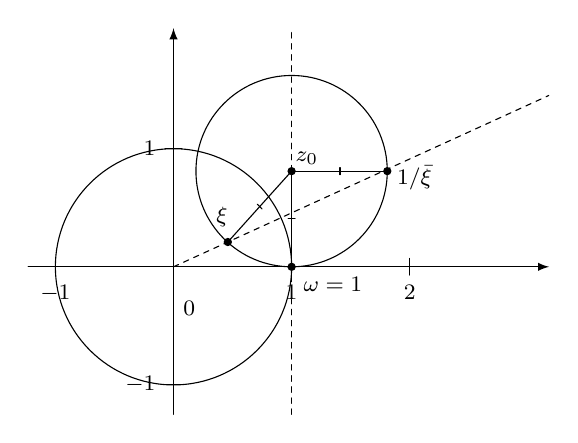
\begin{tikzpicture}[line cap=round,line join=round,>=triangle 45,x=1.0cm,y=1.0cm,scale=1.5]
\draw[-latex,color=black] (-1.23,0) -- (3.18,0);
\foreach \x in {-1,1,2}
\draw[shift={(\x,0)},color=black] (0pt,2pt) -- (0pt,-2pt) node[below] {\footnotesize $\x$};
\draw[-latex,color=black] (0,-1.25) -- (0,2.02);
\foreach \y in {-1,1}
\draw[shift={(0,\y)},color=black] (2pt,0pt) -- (-2pt,0pt) node[left] {\footnotesize $\y$};
\draw[color=black] (0pt,-10pt) node[right] {\footnotesize $0$};
\clip(-1.23,-1.25) rectangle (3.18,2.02);
\draw(0,0) circle (1cm);
\draw [dash pattern=on 2pt off 2pt] (1,-1.25) -- (1,2.02);
\draw(1,0.81) circle (0.81cm);
\draw (1,0.81)-- (0.46,0.21);
\draw (0.75,0.49) -- (0.71,0.53);
\draw (1,0.81)-- (1.81,0.81);
\draw (1.41,0.84) -- (1.41,0.78);
\draw (1,0)-- (1,0.81);
\draw (0.97,0.41) -- (1.03,0.41);
\draw [dash pattern=on 2pt off 2pt,domain=0.0:3.178486501453343] plot(\x,{(-0--0.21*\x)/0.46});
\begin{footnotesize}
\fill (1,0) circle (1pt);
\draw(1.35,-0.15) node {$\omega = 1$};
\fill (0.46,0.21) circle (1pt);
\draw(0.41,0.42) node {$\xi$};
\fill (1.81,0.81) circle (1pt);
\draw(2.04,0.75) node {$1/\bar \xi$};
\fill (1,0.81) circle (1pt);
\draw(1.13,0.92) node {$z_0$};
\end{footnotesize}
\end{tikzpicture}
%\begin{tikzpicture}[line cap=round,line join=round,>=triangle 45,x=1.0cm,y=1.0cm,scale=1.5]
%\draw[-latex,color=black] (-2.02,0) -- (3.23,0);
%\foreach \x in {1}
%\draw[shift={(\x,0)},color=black] (0pt,2pt) -- (0pt,-2pt) node[below right] {\footnotesize $\x$};
%\draw[-latex,color=black] (0,-2.12) -- (0,2.84);
%\foreach \y in {-1}
%\draw[shift={(0,\y)},color=black] (2pt,0pt) -- (-2pt,0pt) node[below left] {\footnotesize $\y$};
%%\draw[color=black] (0pt,-10pt) node[right] {\footnotesize $0$};
%\clip(-2.02,-2.12) rectangle (3.23,2.84);
%\draw(0,0) circle (1cm);
%\draw [dash pattern=on 2pt off 2pt,domain=-2.02:3.23] plot(\x,{(-1-0.19*\x)/-0.98});
%\draw [dash pattern=on 2pt off 2pt,domain=0.0:3.2315706109812745] plot(\x,{(-0--0.27*\x)/0.73});
%\draw [domain=-2.02:3.23] plot(\x,{(--0.2--0.92*\x)/0.71});
%\draw(0.67,1.15) circle (0.88cm);
%\draw (0.67,1.15)-- (0.73,0.27);
%\draw (0.74,0.71) -- (0.66,0.71);
%\draw (0.67,1.15)-- (1.2,0.45);
%\draw (0.97,0.82) -- (0.91,0.77);
%\draw (-0.19,0.98)-- (0.67,1.15);
%\draw (0.23,1.11) -- (0.25,1.03);
%\begin{footnotesize}
%\fill  (-0.19,0.98) circle (1pt);
%\draw (-0.15,1.08) node[left] {$\omega$};
%\fill (0.73,0.27) circle (1pt);
%\draw (0.85,0.18) node {$\xi$};
%\fill  (1.2,0.45) circle (1pt);
%\draw  (1.54,0.36) node {$1/\bar \xi$};
%\fill  (0,0) circle (1pt);
%\fill  (0.67,1.15) circle (1pt);
%\draw (0.55,1.25) node {$z_0$};
%\end{footnotesize}
%\end{tikzpicture}
\end{center}
\caption{A diagram illustrating the statement.} \label{geometry_problem}
\end{figure}
\renewcommand{\CC}{\mathcal C}

Without loss of generality, we need only consider the case where $\omega = 1$, by transforming each point in the statement by the isometry given by $T(z) = e^{-i\theta} z$ where $\omega = e^{i\theta}$.  Having proved the statement for $\omega = 1$, we transform back by $T^{-1}(z) = e^{i \theta}z$, and since this map is an isometry, the coincidence and geometric structure is preserved.

Any circle perpendicular to the unit circle at $\omega = 1$ has as its center $1 + ir$ for some $r>0$.  To see this, recall for every line tangent to a circle at some point $\omega$, the line perpendicular to the tangent at $\omega$ passes through the center of the circle.  Hence, for any circle, say $\CC$, perpendicular to the unit circle at $\omega =1$, $\CC$ is tangent to the real axis at $\omega = 1$, and the perpendicular line $\{1 + ir: r>0\}$ passes through the center.  See \figref{geometry_problem}.

Since $\xi \in \CC$, we have
\begin{align*}
  &|\xi - (1+ir)|^2 = r^2 \\
  \iff & |\xi|^2 - \bar \xi(1+ir) - \xi(1-ir) + 1 + r^2 = r^2\\
  \iff & |\xi|^2 - \bar \xi(1+ir) - \xi(1-ir) + 1 \stackrel\dagger= 0.\\
\end{align*}
Now, it will suffice to show $|1/\bar\xi - (1+ir)|^2 = r^2$.  Observe,
\begin{align*}
  |1/\bar\xi - (1+ir)|^2 
  &= |1/\bar\xi|^2 - (1/\xi)(1+ir) - (1/\bar\xi)(1-ir) + 1 + r^2\\
  &= \frac{1 - \bar\xi(1+ir) - \xi(1-ir) + |\xi|^2}{|\xi|^2} + r^2\\
  &\stackrel\dagger= 0 + r^2.
\end{align*}


%Let $\CC$ denote a perpendicular circle through $\omega$ and $\xi$ and center at $z_0$. From plane geometry, there is a unique line tangent to $\SS^1$ passing through $\omega$, say $\ell_0$. Moreover, the unique line tangent to $\CC$ passing through $\omega$ is perpendicular to the line tangent to $\SS^1$, hence it passes through $z_0$. Recall that $\ell_1: = \{ z \in\mathbb C : |\omega - z| = |z - \xi|\}$ defines the perpendicular bisecting line to the line segment between $\omega$ and $\xi$. Since $\omega$ and $\xi$ are in $\CC$, $z_0 \in \ell_1$. Thus, $z_0 \in \ell_0 \cap \ell_1$.  Since $\omega \notin \ell_1$ (otherwise $\xi = \omega$), $\ell_0$ and $\ell_1$ are distinct lines.  Since lines intersect uniquely, $z_0$ is uniquely determined, and thus $\CC$ is unique.  
\end{solution}

\problem{{\bf D'Angelo 1.17} Prove that the series 
$$
e^M = \sum_{k=0}^\infty \frac{M^k}{k!}
$$
converges for each square matrix of complex numbers.}

  (Please forgive the use of $i$ as an integer index in the following solution.)
\begin{solution}
Let $M$ be a $k\times k$ matrix with entries $\{a_{ij}\}$. Take $m = \max |a_{ij}|$.  We first find an upper bound on the absolute value of the terms of $M^n$ in terms of $|m|$.  We claim such an upper bound is $ k^{n-1}m^n $ and prove it by induction.  By definition, the entries of $M^1$ satisfy $|a_{ij}| \le k^0 m$.  Now, denote the entries of $M^n$ as $b_{ij}(n)$ and suppose $|b_{ij}(n)| \le k^{n-1}m^n$. The absolute value of the $(i,j)$th entry of $M^{n+1}$ is
  $$
    \left|\sum_{s=0}^k b_{is}(n) a_{sj}\right| \le \sum_{s=0}^k |b_{is}(n)| |a_{sj}| \le \sum_{s=0}^k k^{n-1}m^n \cdot m = k^nm^{n+1}.
  $$
  The induction on the claim is complete. Now, the absolute value of the entries of $\sum_{n=0}^N M^n /(n!)$ satisfy
  \begin{align*}
    \left|\sum_{n=0}^N \frac{b_{ij}(n)}{n!}\right| 
    &\le \sum_{n=0}^N \frac{b_{ij}(n)}{n!} \\
    &\le \sum_{n=0}^N \frac{k^{n-1}m^n}{n!} \\
    &\le \sum_{n=0}^N \frac{(km)^n}{n!}. \\
  \end{align*}
  This last sequence of partial sums converges to $e^{km}$, and thinking of $b_{ij}(n)$ as a function of $(i,j)$, the Weierstrass $M$-test gives the convergence of the entries of the partial matrix sums of $\sum M^n/(n!)$.
\end{solution}

\problem{{\bf D'Angelo 1.22} Find $e^{At}$ if 
$$
  A = \begin{pmatrix}
    \lambda & 1 \\
    0 & \lambda
  \end{pmatrix} 
$$ 
\begin{solution}
Let $A = \Lambda + N$ where
$$
  \Lambda = \begin{pmatrix}
    \lambda & 0 \\
    0 & \lambda
  \end{pmatrix} 
  \quad\text{ and }\quad
  N = \begin{pmatrix}
    0 & 1 \\
    0 & 0
  \end{pmatrix} 
$$
Note that $N^2$ is the zero matrix, so $N^j = 0$ for $j>1$. Now, observe for $n>0$
\begin{align*}
  A^n &= (\Lambda + N)^n \\
  &\stackrel{\dagger}=\sum_{j=0}^n\binom{n}{j} \Lambda^{N-n} N^j\\
  &=\Lambda^n + \Lambda^{n-1}N.
\end{align*}
}
Both $\Lambda^n$ and $\Lambda^{n-1}$ are diagonal matrices with $\lambda^n$ and $\lambda^{n-1}$ on each diagonal, respectively.  We compute
$$ 
  A^n =\Lambda^n + \Lambda^{n-1}N = \begin{pmatrix}
    \lambda^n & n \lambda^{n-1} \\
    0 & \lambda^n,
  \end{pmatrix}
$$ 
so 
\renewcommand{\arraystretch}{1.7}
\begin{align*}
  e^{At} 
  &= \sum_{n=0}^\infty \frac{(At)^n}{n!} \\
  &= I + \sum_{n=1}^\infty \frac {t^n}{n!} \left(\Lambda^n + \Lambda^{n-1} N\right)\\
  &= \begin{pmatrix}
    \ds{\sum_{n=0}^\infty (\lambda t)^n/n!} & \ds{\sum_{n=1}^\infty n t^n \lambda^{n-1}/n!} \\
    0 & \ds{\sum_{n=0}^\infty (\lambda t)^n/n!}
  \end{pmatrix}\\
  &= \begin{pmatrix}
    e^{\lambda t} & t e^{\lambda t} \\
    0 & e^{\lambda t}
  \end{pmatrix}.
\end{align*}
We remark that for a matrix in Jordan form, one proceeds as above, but when one expands the binomial in $\dagger$, higher order powers of $N$ appear. One need only compute a closed form for each $\binom nj \Lambda^{n-j}\sum N^n$, which is relatively easy yet tedious and is not done here. 
\end{solution}

\problem{{\bf D'Angelo 1.19} If $B$ is invertible, prove that $Be^MB^{-1} = e^{BMB^{-1}}$.}
\begin{solution}
First note that $(BMB^{-1})^n = BM^nB^{-1}$. This can be seen by induction.  That is, in the $n=1$ case it is given, and if $(BMB^{-1})^n = BM^nB^{-1}$, then $(BMB^{-1})^{n+1} = (BM^nB^{-1})(BMB^{-1}) = BM^{n+1}B^{-1}$, and the induction is complete.  Now, let us compute
\begin{align*}
  e^{BMB^{-1}} 
  &= \sum_{n=0}^\infty (BMB^{-1})^n/n! \\
  &= \sum_{n=0}^\infty BM^nB^{-1}/n! \\
  &= B\left(\sum_{n=0}^\infty M^n/n!\right)B^{-1} \\
  &= Be^MB. \\
\end{align*}
\end{solution}

\problem{{\bf D'Angelo 1.20} Find a simple expression for $\det(e^M)$ in terms of a trace.}
\begin{solution}
  Recall from linear algebra, that for every $k\times k$ matrix $M$, there exists an invertible $k\times k$ matrix $P$, and an upper triangular matrix $U$ so that 
  $$
    M = PUP^{-1}.
  $$
  %Using various properties of determinants, we have
  %$$
  %  \det M = \det(PUP^{-1}) = \det(P)\det(U)\det(P)^{-1} = \det(U),
  %$$
  %of which on the far right hand side, the determinant is given by the product of the diagonal elements of $U$.  
  Using the result in 1.19, we have
  $$
   e^M = Pe^{U}P^{-1}. 
  $$
  Note that for $U$ upper triangular with diagonal elements
  $(\lambda_1,\dots,\lambda_k)$, $U^n$ is also upper triangular with diagonal
  elements $(\lambda_1^n,\dots,\lambda_k^n)$. Hence, $e^U$ is upper triangular
  with diagonal elements $(e^{\lambda_1},\dots,e^{\lambda_k})$. Using the fact
  that the determinant of an upper triangular matrix is given by the product of
  the diagonal elements, and that determinants respect multiplication and
  inversion, we have
  $$
    \det(e^M) = \det(P)\det(e^U)\det(P)^{-1} = \prod_{j=1}^k e^{\lambda_j} = \exp\left(\sum_{j=1}^k \lambda_j\right) = \exp(\mathrm{Tr(M)}),
  $$
  where $\mathrm{Tr}(M)$ denotes the trace of $M$.
\end{solution}

\end{document}
